\chapter{Arhitektura i dizajn sustava}
		


	
	Arhitektura aplikacije može se podijeliti na 3 djela. 
	
	\begin{packed_item}
		\item web poslužitelj
		
		\item web preglednik
		
		\item baza podataka
	
	\end{packed_item}
	
	\underbar{Web preglednik} je program koji korisniku omogućuje pristup web stranicama te multimedijskom sadržaju na njima. Web preglednik omogućuje korisniku pristup web poslužitelju putem HTTPS (eng. \textit{Hypertext Transfer Protokol Secure}) protokola te interpretira sadržaj kojeg je poslao Web poslužitelj u ljudski razumljiv oblik.
	
	\underbar{Web poslužitelj} je program koji prima i odgovara na korisnikove HTTPS zahtjeve. Web poslužitelj pokreće aplikaciju te korisniku šalje potrebne podatke kako bi korisnikov web preglednik mogao generirati frotnend aplikacije. Frontend predstavlja korisničko sučelje te je pisan u HTML-u, CSS-u i JavaScriptu uz pomoć React framework-a. ReactJS je biblioteka čiji su glavni element komponente. Komponente unutar sebe sadržavaju dijelove korisničkog sučelja te opisuju njihovo ponašanje. Glavna prednost korištenja komponenti je što se one mogu ponovno koristiti te se nove složenije komponente mogu spajati u složenije. Ovakav modularan pristup dizajniranju korisničkog sučelja čini nadogradnju i promjenu korisničkog sučelja vrlo jednostavnom. React dodatno sadrži virtualan DOM kojim optimizira rad korisničkog sučelja tako što minimizira broj manipulacija stvarnog DOM-a. Web poslužitelj je pisan u programskom jeziku Java i Spring Boot radnom okviru. Web poslužitelj komunicira sa bazom podataka te šalje podatke iz nje korisniku u prikladnom obliku. Spring Boot je radno sučelje za brz i učinkovit razvoj WEB aplikacija. Drži se principa konvencija iznad konfiguracije (engl. convention over configuration), to znači da Spring Boot oduzima mogućnost potpuno kontrole nad funkcioniranjem sustava od korisnika no zauzvrat pojednostavljuje razvoj web poslužitelja. Spring Boot ima višeslojnu  arhitekturu gdje se podatci i zahtjevi šalju među raznim slojevima od kojih svaki ima svoju zadaću i logiku. Tako controller sloj prima i obrađuje HTTP zahtijeve, data access sloj komunicira s bazom podataka, exception handling layer je odgovoran za hvatanje i obrađivanje pogreški...
	
	\underbar{Baza podataka} implementirana je putem PostgresSQL-a. Sadrži podatke potrebne za funkcioniranje aplikacije te njihove međusobne odnose. 

	
		

	
				
		\section{Baza podataka}
			
		Baza podataka za web aplikaciju koristi relacijski model podataka. Kao RDBMS (Relational Database Management System) koristi se PostgreSQL verzija 15.0. Koristeći ERDPlus, stvaramo ER dijagram baze podataka u kojem navodimo sve entitete, njihove atribute te međusobne veze. Daljnje tipove podataka, primarne, strane i alternativne ključeve navodimo u relacijskoj shemi baze podataka.
		
			
			\subsection{Opis tablica}
				%\textbf{Employee}]
				Employee  Ovaj entitet sadržava sve važne informacije o zaposleniku koji koristi aplikaciju. Sadrži atribute: id, first\_name, last\_name, email, password i role. Ovaj entitet u vezi je One-to-Many s entitetom Photos preko zaposlenikovog id-a te je u vezi One-to-Many s entitetom Document preko zaposlenikovog id-a.
			
		
				\begin{longtblr}[
					label=none,
					entry=none
					]{
						width = \textwidth,
						colspec={|X[6,l]|X[7, l]|X[20, l]|}, 
						rowhead = 1,
					} %definicija širine tablice, širine stupaca, poravnanje i broja redaka naslova tablice
					\hline \SetCell[c=3]{c}{\textbf{Employee}}	 \\ \hline[3pt]
					\SetCell{LightGreen}id & BIGINT	&  	Jedinstveni identifikator svakog zaposlenika  	\\ \hline
					first\_name	& VARCHAR(255) &   Ime zaposlenika	\\ \hline
                    last\_name & VARCHAR(255) &   Prezime korisnika    \\ \hline 
					role & VARCHAR(255) &   Funkcija svakog zaposlenika (limitirano na Zaposlenik, Revizor, Računovođa i Direktor)   \\ \hline 
					password & VARCHAR(255)	&  	Zaposlenikova hashirana lozinka  	\\ \hline 
					email & VARCHAR(255)   &   E-mail korisnika \\ \hline
				\end{longtblr}
				
				\textbf{Photos}  Ovaj entitet sadržava sve važne informacije o fotografijama pohranjenima u bazu. Sadrži atribute: photoid, url, image\_name, upload\_time te strani ključ upload\_employee\_id preko korisnika. Ovaj entitet u vezi je Many-to-One s entitetom Employee preko zaposlenikovog id-a te je u One-to-One vezi s entitetom Document koji sadrži strani ključ photo\_id.

				\begin{longtblr}[
					label=none,
					entry=none
					]{
						width = \textwidth,
						colspec={|X[11,l]|X[8, l]|X[20, l]|}, 
						rowhead = 1,
					}
					\hline \SetCell[c=3]{c}{\textbf{Photos}}	 \\ \hline[3pt]
					\SetCell{LightBlue} upload\_employee\_id	& BIGINT   &   Jedinstveni identifikator zaposlenika koji je objavio fotografiju izveden iz tablice Employee	\\ \hline
                    \SetCell{LightGreen} photo\_id  & BIGINT   &   Jedinstveni identifikator fotografije \\ \hline
                    url   & VARCHAR(255)   &  URL fotografije \\ \hline
                    image\_name   & VARCHAR(255)  &  Ime prenesene fotografije \\ \hline
                    upload\_time  & TIMESTAMP  &  Datum i vrijeme prijenosa fotografije \\ \hline
				\end{longtblr}

				\textbf{Document}  Ovaj entitet sadržava sve važne informacije o dokumentima pohranjenima u bazi. Sadrži atribute: id, correct, type, to\_be\_signed, signed, verified, url, file\_name te strane ključeve photo\_id, scan\_employee\_id i verification\_employee\_id. Ovaj entitet u vezi je One-to-One s entitetom Photos preko photo\_id, u Many-to-One vezi je s entitetom Employee te je u vezi One-to-One s entitetom Archive koji sadrži document\_id kao strani ključ.

                \begin{longtblr}[
					label=none,
					entry=none
					]{
						width = \textwidth,
						colspec={|X[17,l]|X[10, l]|X[20, l]|}, 
						rowhead = 1,
					}
					\hline \SetCell[c=3]{c}{\textbf{Document}}	 \\ \hline[3pt]
                    \SetCell{LightBlue} photo\_id  &  BIGINT  &  Jedinstveni identifikator fotografije sadržane u dokumentu, izveden iz tablice Photos	\\ \hline
					\SetCell{LightBlue} scan\_employee\_id  &  BIGINT  &  Jedinstveni identifikator zaposlenika koji je skenirao dokument izveden iz tablice Employee	\\ \hline
					\SetCell{LightBlue} verification\_employee\_id  &  BIGINT  &  Jedinstveni identifikator zaposlenika zaduženog za verifikaciju ispravnosti konverzije, izveden iz tablice Employee	\\ \hline
                    \SetCell{LightGreen} id  &  BIGINT  &  Jedinstveni identifikator prenesenog dokumenta \\ \hline
                    correct  &  BOOLEAN  &  Potvrda ukoliko je rezultantni dokument ispravno skeniran \\ \hline
                    type  &  VARCHAR(255)  &  Tip dokumenta (limitirano na Račun, Ponuda i Interni dokument) \\ \hline
                    signed  &  BOOLEAN  &  Potvrda ukoliko je rezultantni dokument potpisan od strane direktora \\ \hline
                    verified  &  BOOLEAN  &  Potvrda ukoliko je rezultantni dokument potpisan od strane računovođe \\ \hline
                    to\_be\_signed  &  BOOLEAN  &  Potvrda ukoliko rezultantni dokument očekiva potpis od direktora\\ \hline
					file\_name  &  VARCHAR(255)  &  Ime pohranjenog dokumenta\\ \hline
					url  &  VARCHAR(255)  &  URL zapis\\ \hline
                \end{longtblr}

				\textbf{Archive\_entity}  Ovaj entitet sadržava sve važne informacije o arhiviranim dokumentima u bazi. Sadrži atribute: id te strani ključ document\_id preko entiteta Dokument. Ovaj entitet u vezi je One-to-One s entitetom Dokument preko dokumentovog id-a.

                \begin{longtblr}[
					label=none,
					entry=none
					]{
						width = \textwidth,
						colspec={|X[6,l]|X[6, l]|X[20, l]|}, 
						rowhead = 1,
					}
					\hline \SetCell[c=3]{c}{\textbf{Archive}}	 \\ \hline[3pt]
                    \SetCell{LightBlue} document\_id  &  BIGINT  &  Jedinstveni identifikator dokumenta koji se arhivira \\ \hline
                    \SetCell{LightGreen} id  &  BIGINT  &  Jedinstveni identifikator dokumenta koji se nalazi u arhivi \\ \hline
                \end{longtblr}

				\textbf{Login\_log\_out\_record}  Ovaj entitet sadržava sve važne informacije o vremenu rada svakog pojedinačnog zaposlenika. Sadrži atribute: id, login\_time, logout\_time te strani ključ employee\_id preko korisnikovog identifikatora. Ovaj entitet je u vezi Many-to-One s entitetom Employee preko zaposlenikovog id-a.

				\begin{longtblr}[
					label=none,
					entry=none
					]{
						width = \textwidth,
						colspec={|X[6,l]|X[6, l]|X[20, l]|}, 
						rowhead = 1,
					}
					\hline \SetCell[c=3]{c}{\textbf{Login/Logout records}}	 \\ \hline[3pt]
                    \SetCell{LightBlue} employee\_id  &  BIGINT  &  Jedinstveni identifikator zaposlenika čija se aktivnost na stranici sprema u statistiku \\ \hline
					\SetCell{LightGreen} id  &  BIGINT  &  Jedinstveni identifikator session-a koji se gleda \\ \hline
                    login\_time  &  TIMESTAMP  &  Datum i vrijeme login-a zaposlenika \\ \hline
					logout\_time &  TIMESTAMP  &  Datum i vrijeme logout-a zaposlenika \\ \hline
                \end{longtblr}

			\subsection{Dijagram baze podataka}
				
				\begin{figure}[H]
					%\includegraphics[scale=0.6]{slike/kompletici_v4RE.png} %veličina slike u odnosu na originalnu datoteku i pozicija slike
					\centering
					\caption{ER dijagram baze podataka}
					\label{fig:promjene}
				\end{figure}
				
					\begin{figure}[H]
					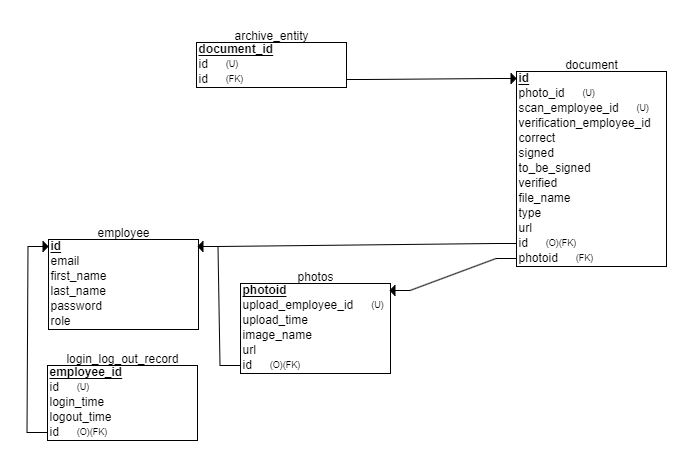
\includegraphics[scale=0.5]{slike/kompletici_v4_REL.PNG} %veličina slike u odnosu na originalnu datoteku i pozicija slike
					\centering
					\caption{REL dijagram baze podataka}
					\label{fig:promjene}
				\end{figure}
				
				
			
			\eject
			
			
		\section{Dijagram razreda}

		Na slikama su prikazani razredi koji pripadaju backend dijelu arhitekture. Na slikama su prikazani razredi koji nasljeđuju Controller razred, metode pomoću kojih oni manipuliraju s DTO (Data transfer objects), te razredi koji implementiraju razred Entity.
		
			\begin{figure}[H]
				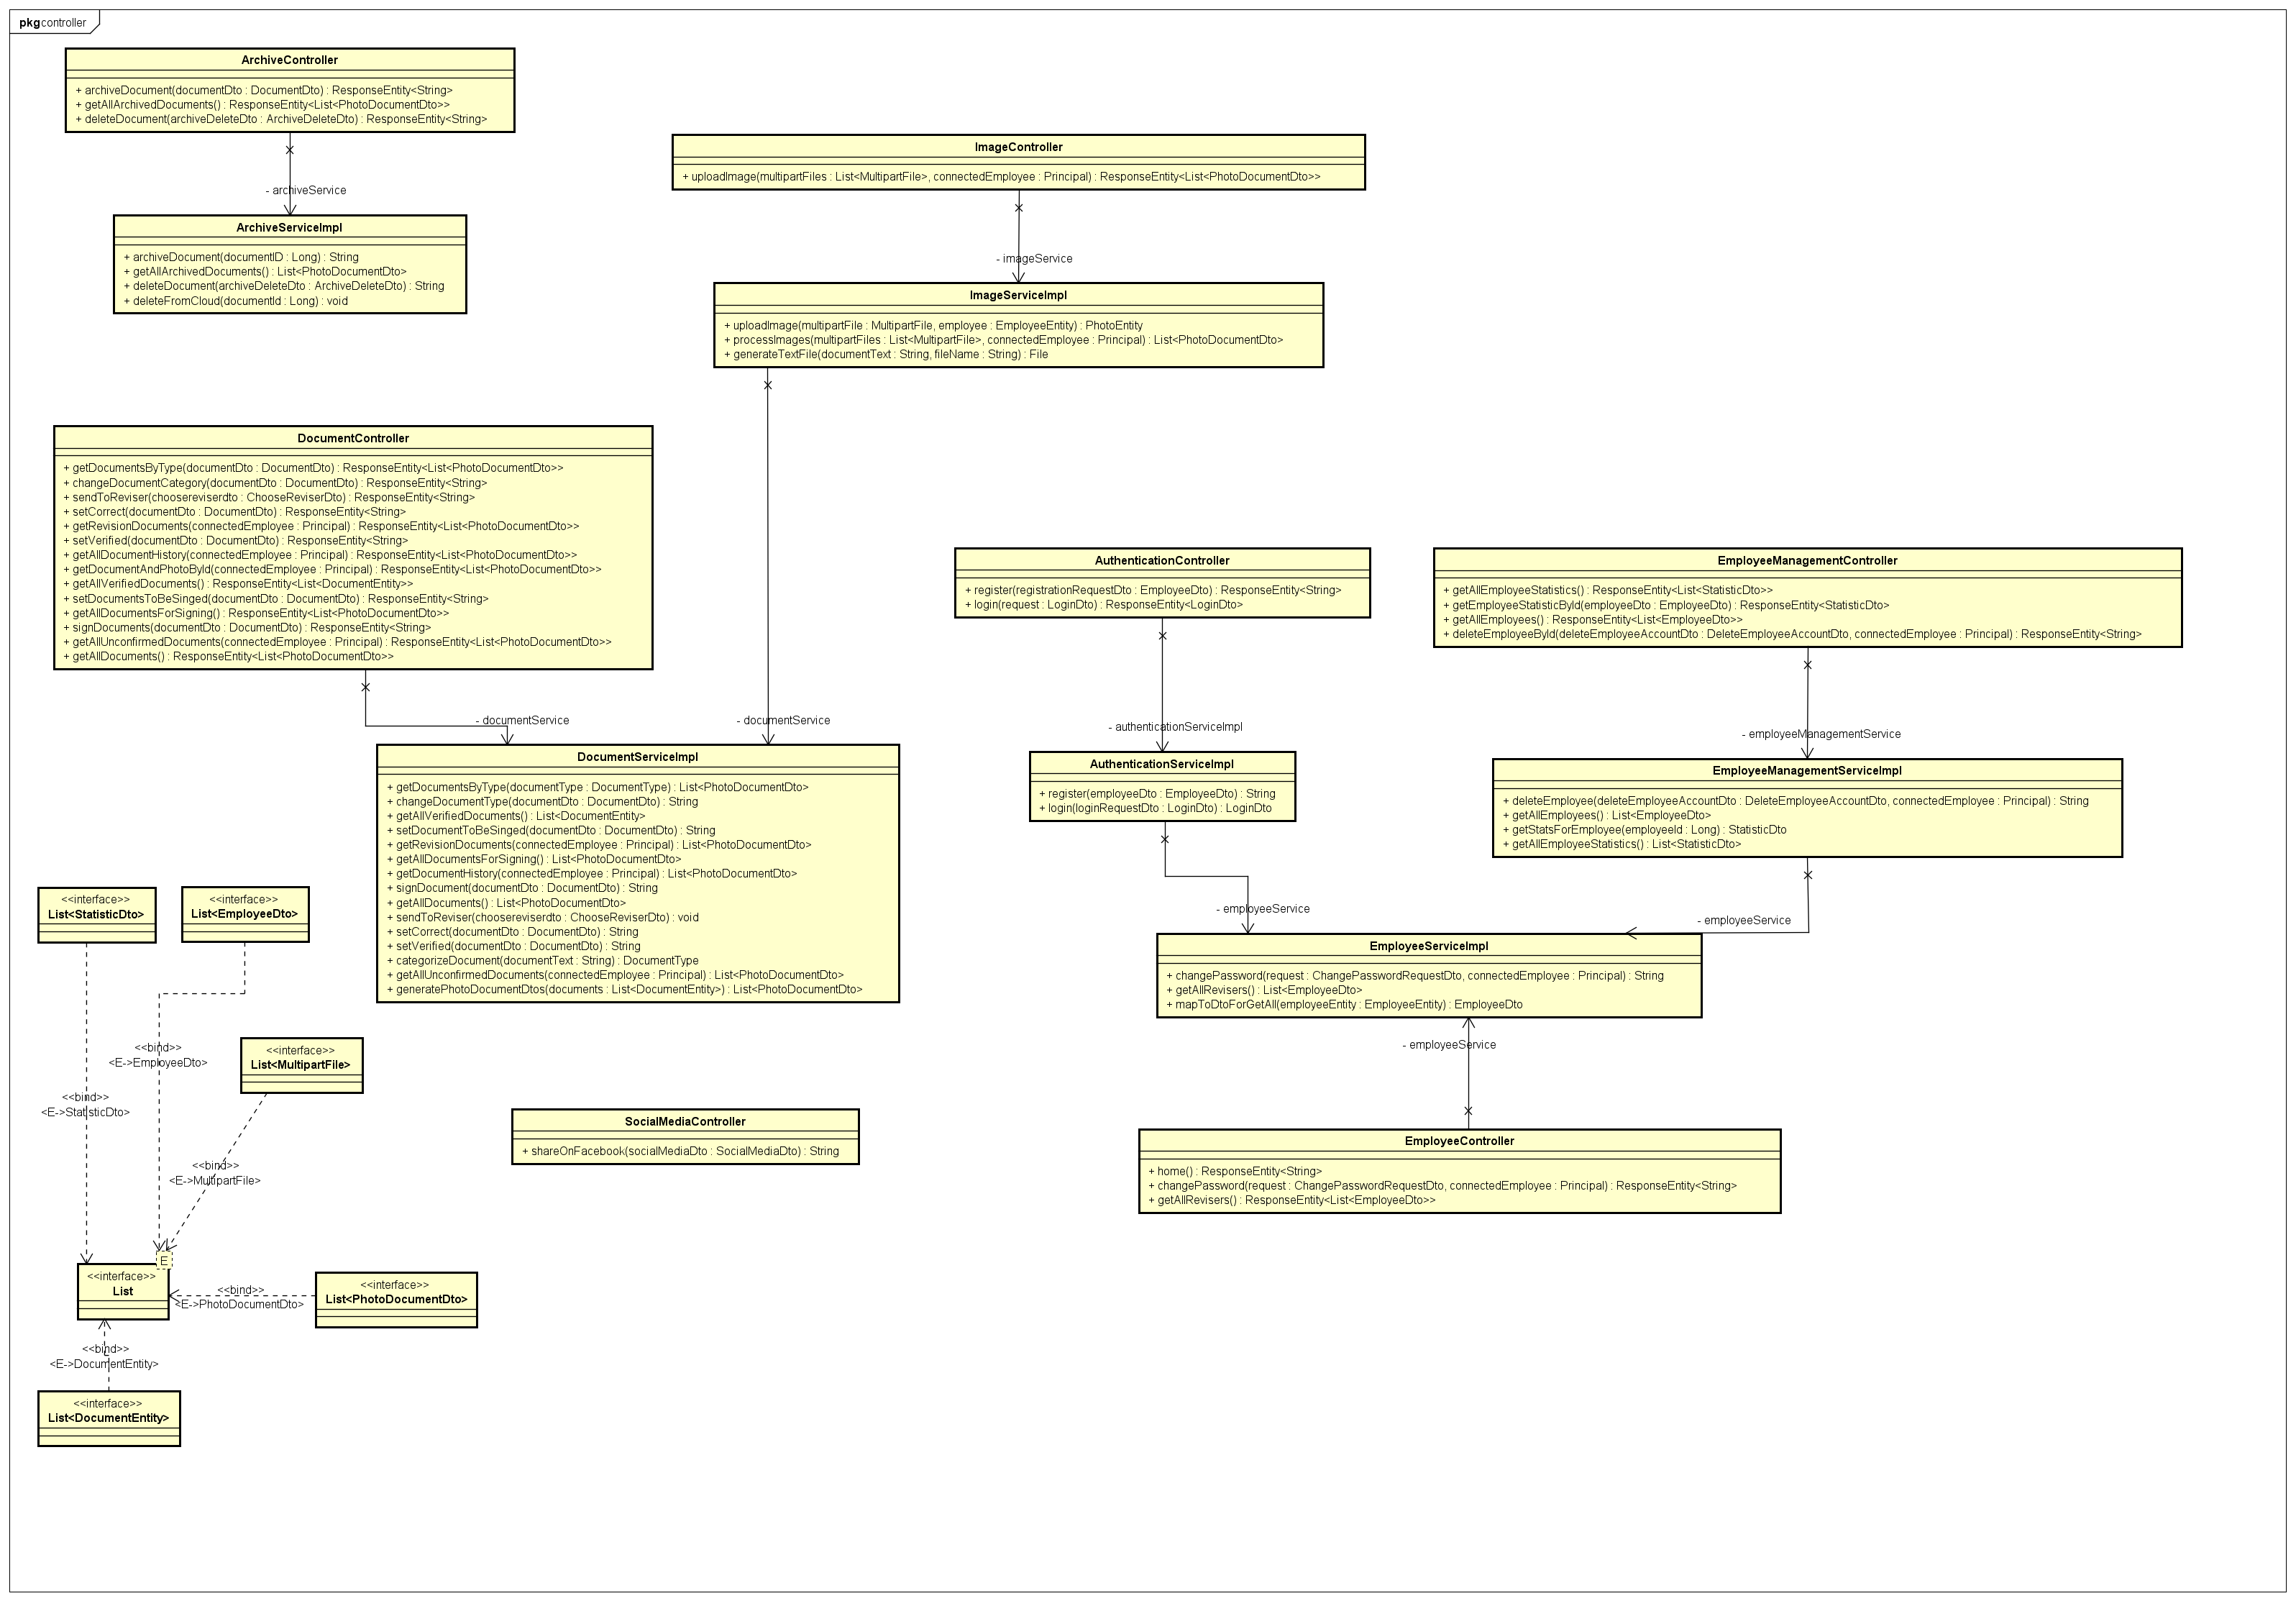
\includegraphics[scale=0.2]{slike/ControlerDiagram.png} %veličina slike u odnosu na originalnu datoteku i pozicija slike
				\centering
				\caption{Dijagram razreda - dio Controllers}
				\label{fig:promjene}
			\end{figure}
			
			\begin{figure}[H]
				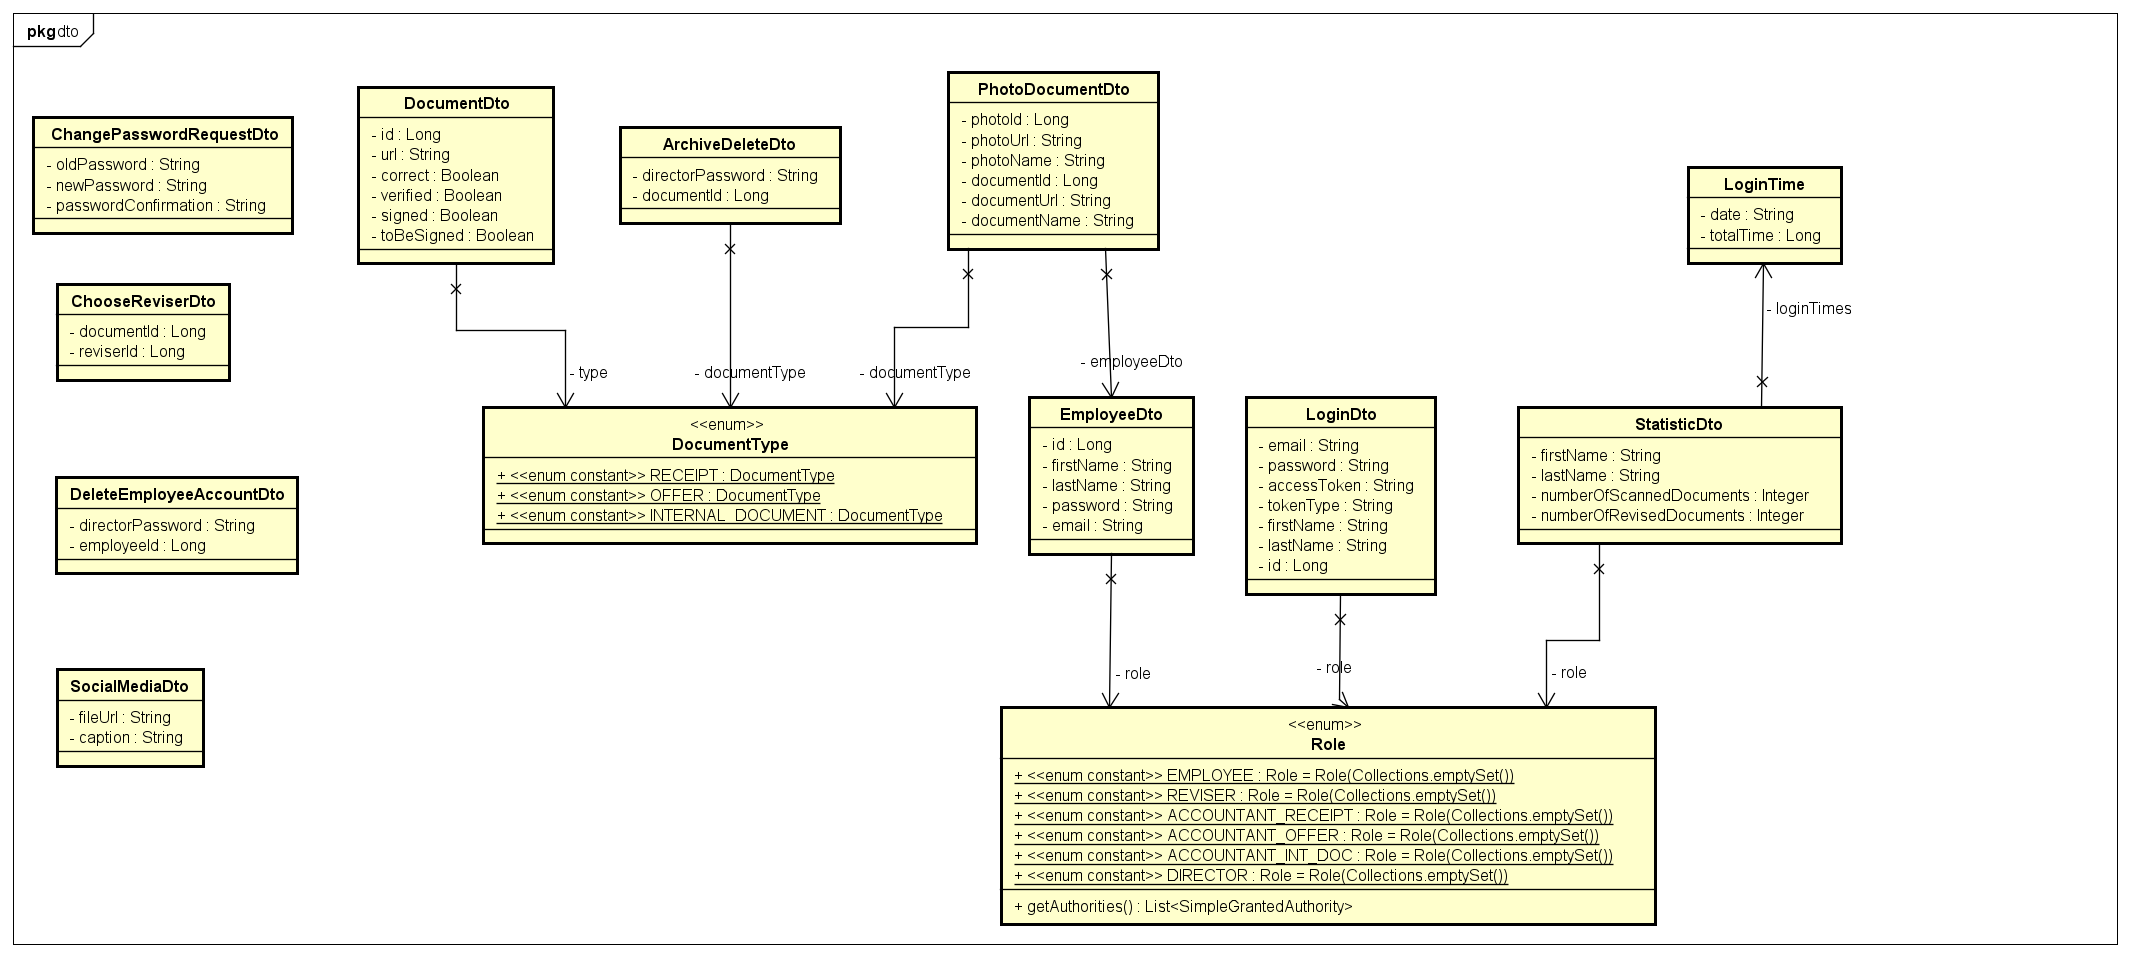
\includegraphics[scale=0.3]{slike/DtoDiagram.png} %veličina slike u odnosu na originalnu datoteku i pozicija slike
				\centering
				\caption{Dijagram razreda - dio Data transfer objects}
				\label{fig:promjene}
			\end{figure}

			\begin{figure}[H]
				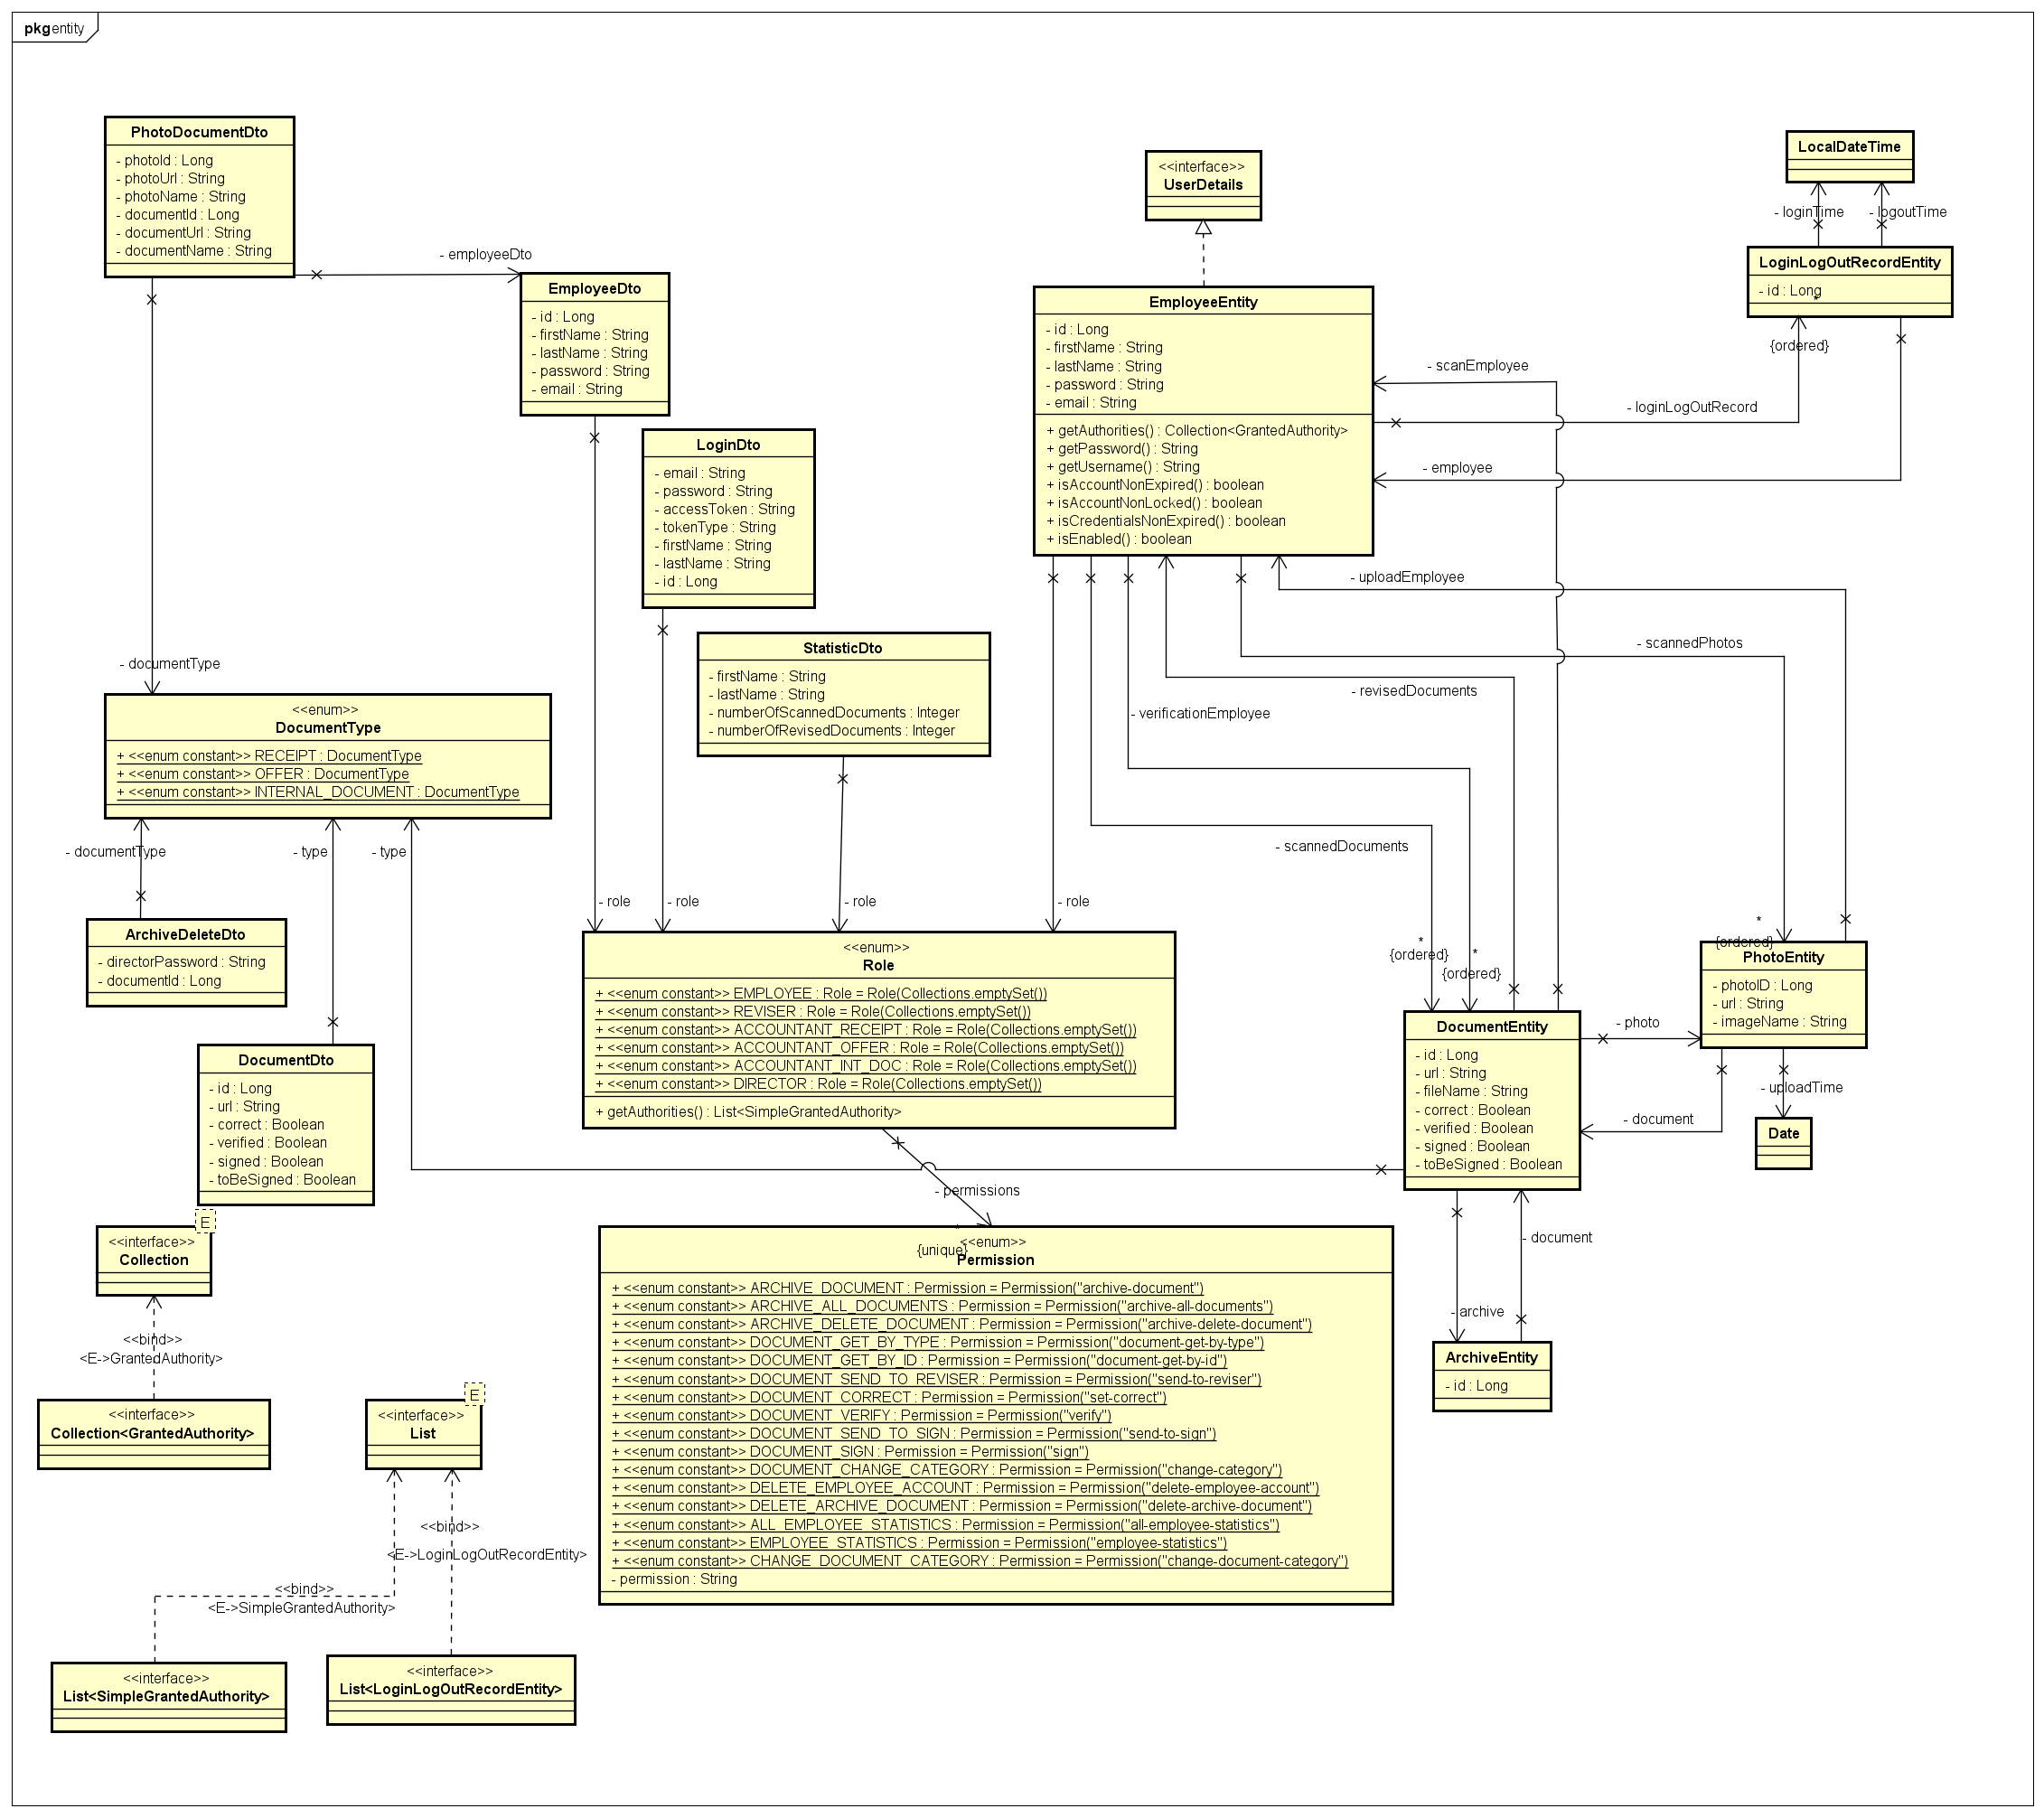
\includegraphics[scale=0.3]{slike/EntityDiagram.png} %veličina slike u odnosu na originalnu datoteku i pozicija slike
				\centering
				\caption{Dijagram razreda - dio Entity}
				\label{fig:promjene}
			\end{figure}
			
			
			
			\eject
		

		\section{Dijagram stanja}
			
			Dijagram stanja prikazuje stanja objekta te prijelaze iz jednog stanja u drugo temeljene na dogadajima. Na slici je prikazan dijagram stanja za direktora. Nakon prijave, direktoru se prikazuje početna stranica na kojoj može pristupit svim svojim funkcionalnostima (skeniranju dokumenata, promjeni lozinke, pregledu zahtjeva itd.). Odabirom na skeniranje dokumenata direktoru se pruža mogućnost odabira upload-a dokumenta ili provjere već dostupnog dokumenta. Odabirom pregleda zahtjeva pružaju mu se opcije revizije, potpisivanja te arhiviranja dokumenta. Odabirom pregleda zapisa direktor može pregledati arhivu, povijest skeniranja te statistiku svih pojedinačnih zaposlenika. Direktoru se također pružaju opcije promjene lozinke, brisanja zaposlenika te objave dokumenta na društvenim mrežama (u ovom slučaju na društvenoj mreži "Facebook").
			
			\begin{figure}[H]
				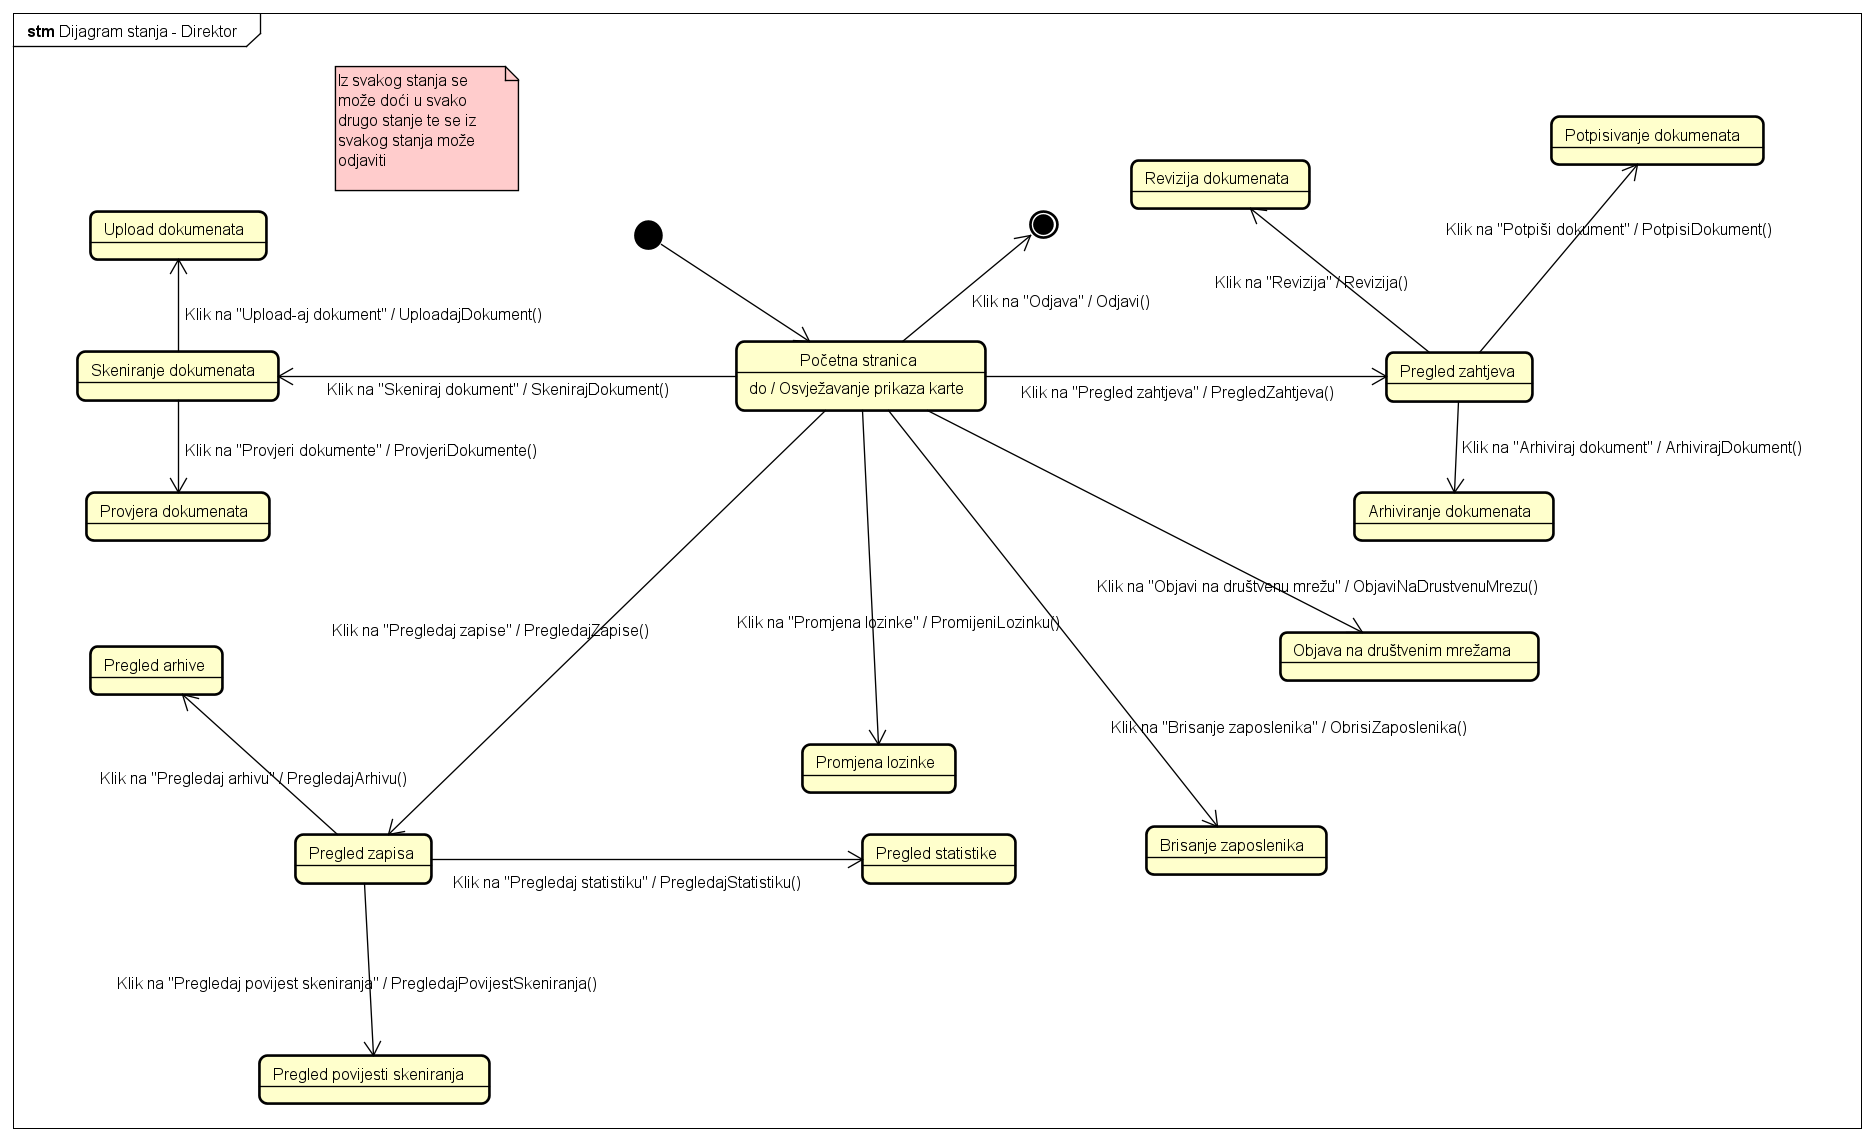
\includegraphics[scale=0.35]{slike/DijagramStanja - Direktor.png} %veličina slike u odnosu na originalnu datoteku i pozicija slike
				\centering
				\caption{Dijagram stanja}
				\label{fig:promjene}
			\end{figure}

			\eject 
		
		\section{Dijagram aktivnosti}
			
			
			Dijagram aktivnosti primjenjuje se za opis modela toka upravljanja ili toka podataka. Ne upotrebljava se za modeliranje događajima poticanog ponašanja. U modeliranju toka upravljanja svaki novi korak poduzima se nakon završenog prethodnog, a naglasak je na jednostavnosti. Na dijagramu aktivnosti prikazan je princip rada zaposlenika. Zaposlenik nakon uspješne prijave u sustav upload-a fotografije koje se daju na skeniranje, te aplikacija iste fotografije konvertira koristeći Tesseract.

			\begin{figure}[H]
				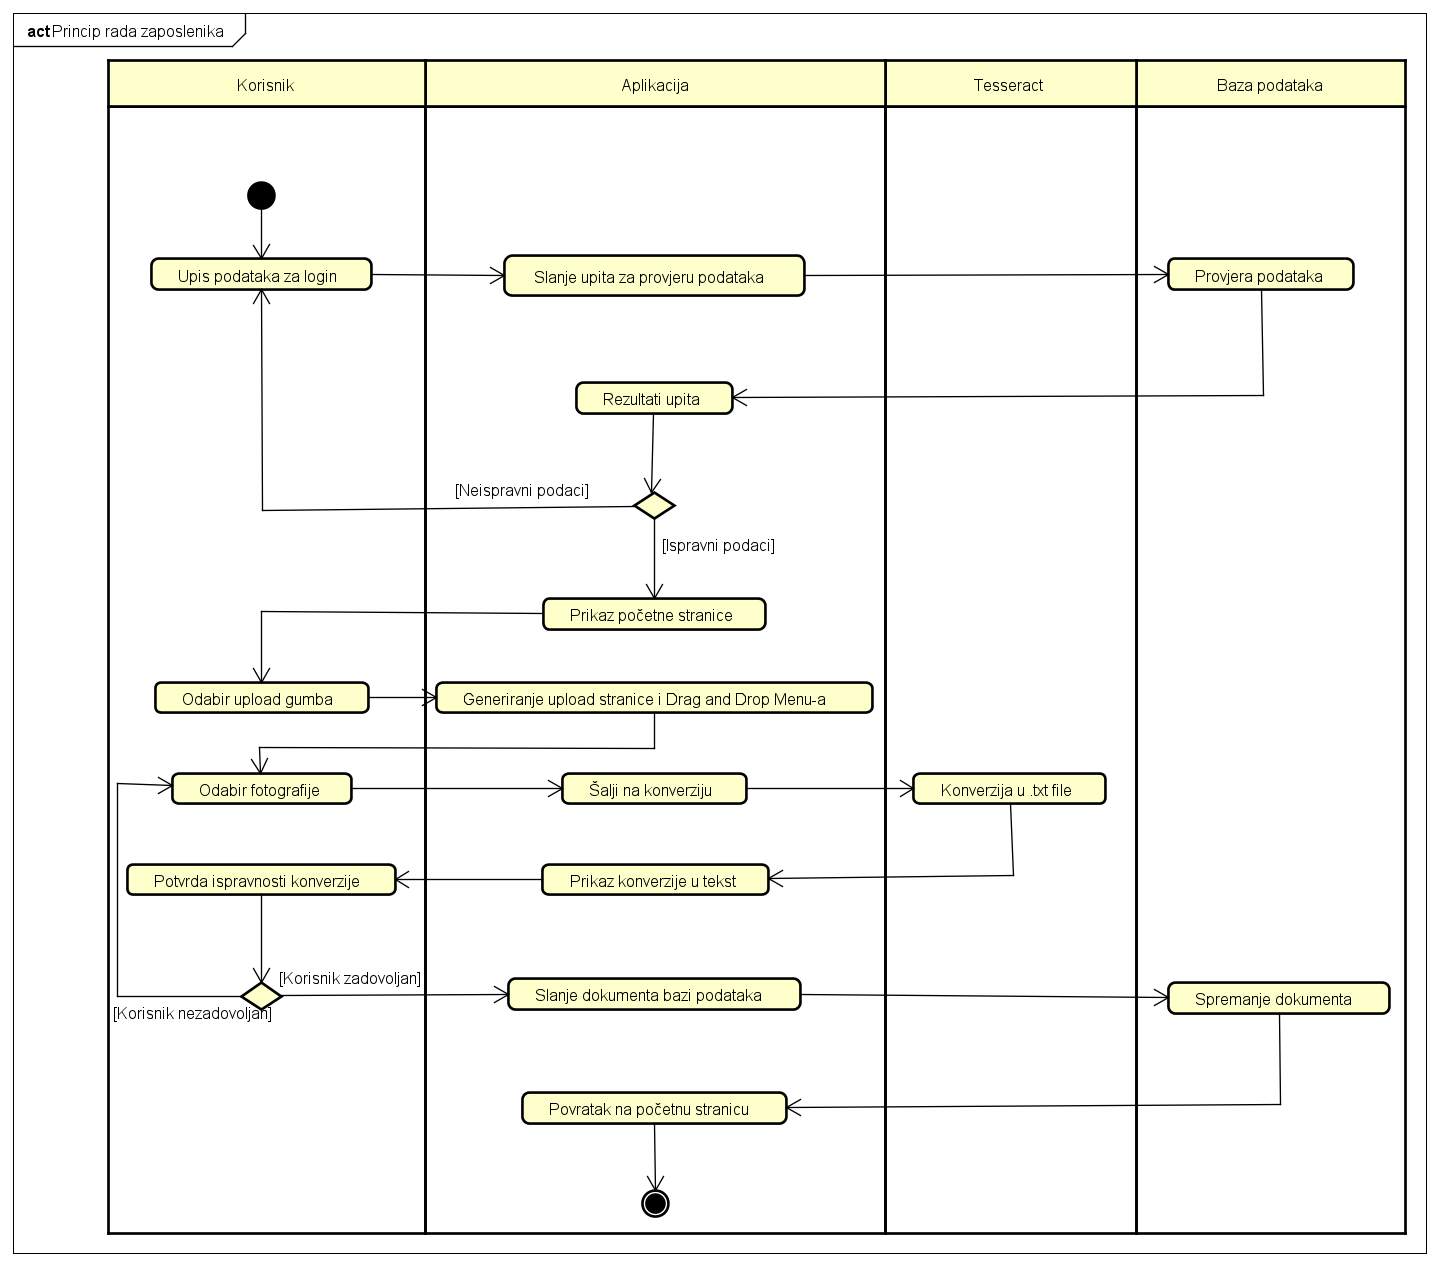
\includegraphics[scale=0.4]{slike/dijagram_aktivnosti.png} %veličina slike u odnosu na originalnu datoteku i pozicija slike
				\centering
				\caption{Dijagram aktivnosti}
				\label{fig:promjene}
			\end{figure}


			\eject
		\section{Dijagram komponenti}
		
			
			 Dijagram komponenti prikazan na slici opisuje organizaciju i međuovisnost komponenti, interne strukture i odnose prema okolini. Sustavu se pristupa preko dva različita sučelja. Preko sučelja za dohvat HTML, CSS i JS datoteka poslužuju se datoteke koje pripadaju frontend dijelu aplikacije. Router je komponenta koja na upit s url određuje koja datoteka će se poslužiti na sučelje. Frontend dio se sastoji od niza JavaScript datoteka koje su raspoređene u logičke cjeline nazvane po tipovima aktora koji im pristupaju. Sve JavaScript datoteke ovise o React biblioteci iz koje dohvaćaju gotove komponente kao što su gumbi, forme i slično. Preko sučelja za dohvat JSON podataka pristupa se REST API komponenti. REST API poslužuje podatke koji pripadaju backend dijelu aplikacije. EntityFrameWorkCore je zadužen za dohvaćanje tablica iz baze podataka pomoću SQL upita. Podaci koji su pristigli iz baze se šalju dalje MVC arhitekturi u obliku DTO preko Services. React-view komponenta preko dostupnih sučelja komunicira sa aplikacijom te ovisno o korisnikovim akcijama osvježava prikaz i dohvaća nove podatke ili datoteke.

			 \begin{figure}[H]
				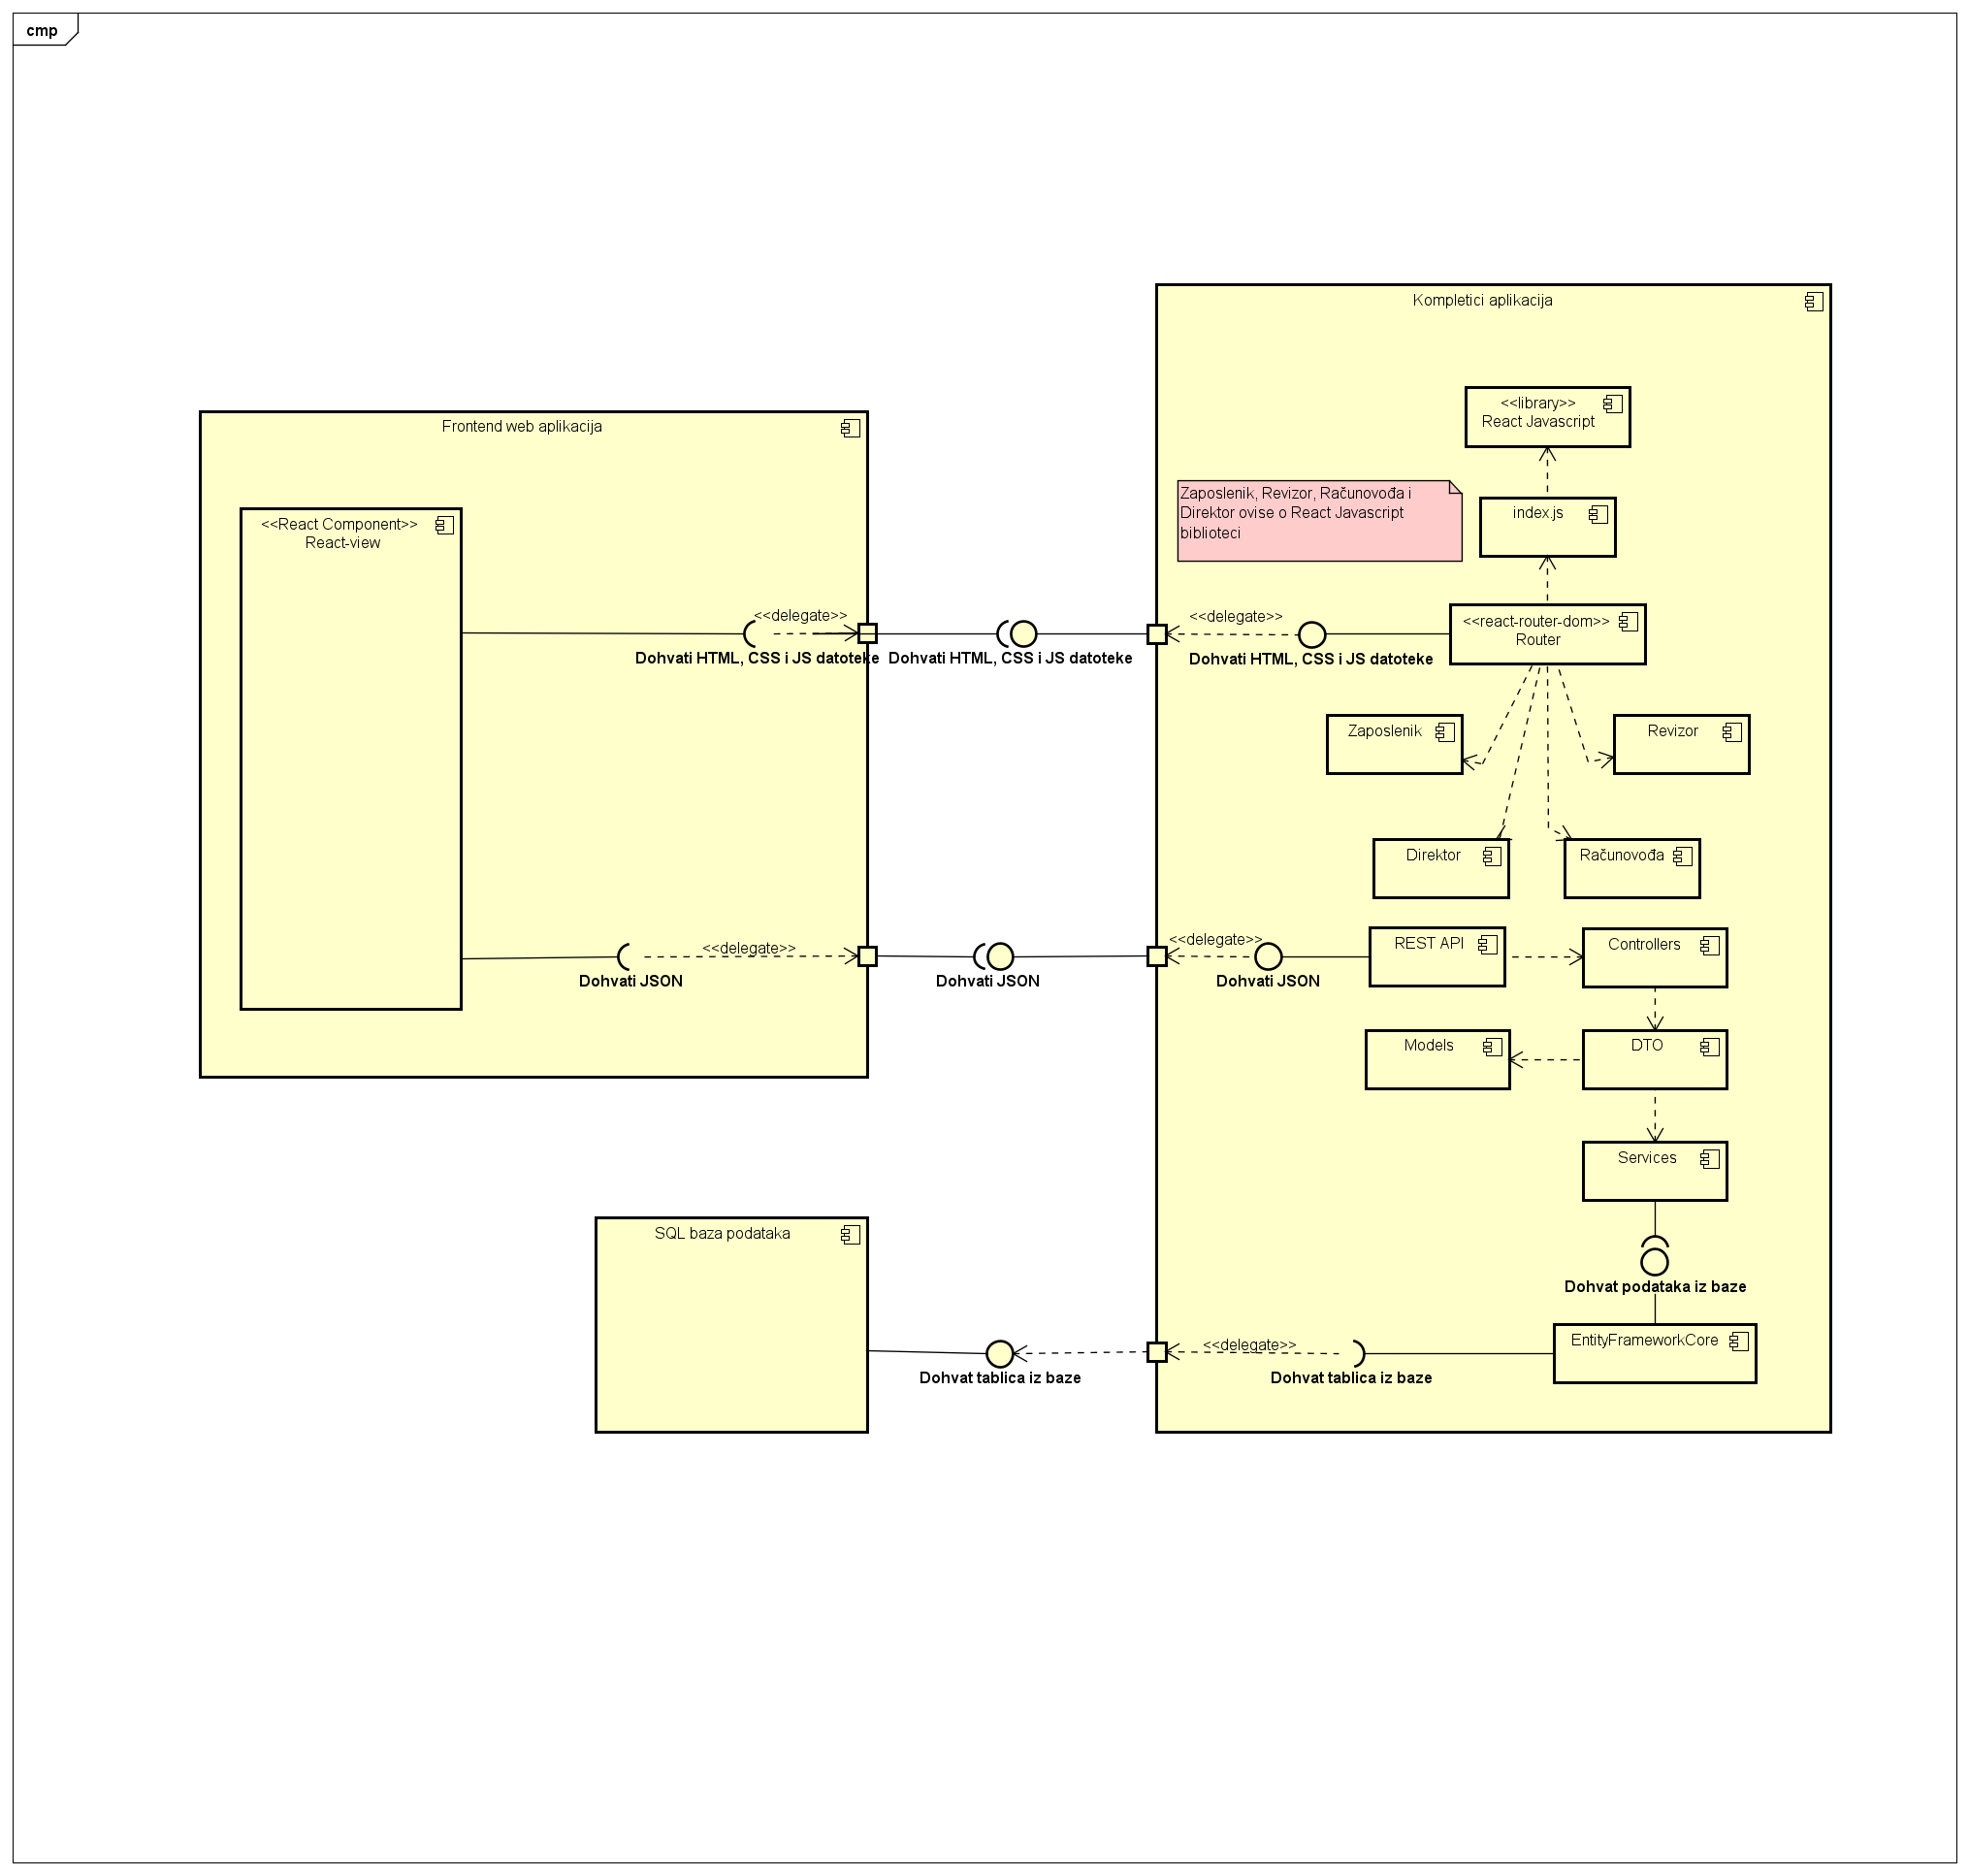
\includegraphics[scale=0.3]{slike/dijagram_komponenti.png} %veličina slike u odnosu na originalnu datoteku i pozicija slike
				\centering
				\caption{Dijagram komponenti}
				\label{fig:promjene}
			\end{figure}
			 
		